
\documentclass[11pt,a4paper]{article}
\usepackage[margin=1in]{geometry}
\usepackage[T1]{fontenc}
\usepackage[utf8]{inputenc}
\usepackage{lmodern}
\usepackage{amsmath}
\usepackage{booktabs}
\usepackage{graphicx}
\usepackage{hyperref}
\usepackage{array}
\usepackage{enumitem}
\usepackage{xcolor}
\hypersetup{colorlinks=true, linkcolor=blue, urlcolor=blue, citecolor=blue}
\setlength{\parskip}{0.55em}
\setlength{\parindent}{0pt}
\renewcommand{\arraystretch}{1.18}

\title{Spherical Cyclic Time v2.0 Addendum\\Minimal Closed-Background Transfer Tests}
\author{Public synthesis addendum}
\date{2026-07-04}

\begin{document}
\maketitle

\begin{abstract}
This addendum summarizes the v2.0-A through v2.0-F branch of Spherical Cyclic Time (SCT). The branch was opened after an external referee-style review argued that v1.7-v1.9 should be treated as requirements and obstruction audits, not as computational negative results. The v2.0 branch therefore refocused on a minimal computational question: whether a preregistered closed toy background can produce a perturbative transfer shape compatible with the Gaussian/diffusive ansatz $\exp[-(k/k_c)^2]$. Two independently preregistered toy background families were tested. Both produced bounded, high-$k$ plateau-like transfer shapes and were classified as non-Gaussian transfer under the locked rules. The result is a limited computational negative result for the tested closed-background route. It is not a no-go theorem for cyclic or bounce cosmology and it is not a physical cosmology or observational claim.
\end{abstract}

\section{Purpose of this addendum}
The previous v1.7-v1.9 line of work mapped requirements and obstructions for turning SCT from an informational toy framework into a more physical open-system or background-transition model. That line was useful as governance, but it did not produce a new computational result. The v2.0 branch was therefore deliberately narrowed to a single computable target:
\[
T_R(k)\quad \hbox{from a closed, preregistered toy background.}
\]

The branch did not attempt to derive a bath, a noise kernel, $P_\xi$, $\Gamma_S$, FDT/KMS conditions, an entropy map, or an observational fit. The only tested question was whether the closed-background transfer shape resembles the Gaussian/diffusive form used as a conditional toy ansatz in earlier versions.

\section{Locked minimal protocol}
The proxy perturbation equation was fixed before execution:
\[
 u_k''+\left(k^2-\frac{a''}{a}\right)u_k=0.
\]
The mode grid was fixed as
\[
 k=\operatorname{logspace}(-2,2,121), \qquad y\in[-50,50].
\]
The transfer shape was extracted using the preregistered two-basis norm protocol. The Gaussian comparison
\[
 T_G(k)=\exp[-(k/k_c)^2]
\]
was used only as a diagnostic comparator, not as a target for tuning.

\section{Background families tested}
Two background families were preregistered and then executed.

\textbf{Family 1: smooth global power bounce.}
\[
 a(y)=(1+y^2)^{\alpha/2}.
\]
Primary value: $\alpha=0.20$. Sensitivity values: $\alpha=0.10$ and $\alpha=0.50$.

\textbf{Family 2: compact $C^2$ matched power-law bounce.}
For $|y|\geq 1$,
\[
 a(y)=|y|^\alpha.
\]
For $|y|<1$,
\[
 a(y)=a_0+b y^2+c y^4,
\]
with
\[
 c=\frac{\alpha(\alpha-2)}{8},\qquad
 b=\frac{\alpha(4-\alpha)}{4},\qquad
 a_0=1-\frac{\alpha(6-\alpha)}{8}.
\]
The same primary and sensitivity values were used.

\section{Results}
All six executed cases were classified as non-Gaussian transfer under the locked rules. The primary results are shown below.

\begin{center}
\begin{tabular}{p{0.30\linewidth}cccc}
\toprule
Background family & $\alpha$ & $T_{\min}$ & high-$k$ plateau & Gaussian $R^2$ \\
\midrule
Smooth global power bounce & 0.20 & 0.496693 & 0.496709 & -3.337 \\
Compact $C^2$ matched bounce & 0.20 & 0.484690 & 0.484705 & -2.021 \\
\bottomrule
\end{tabular}
\end{center}

The sensitivity cases gave the same qualitative classification: non-Gaussian transfer with bounded/high-$k$ plateau behavior.

\begin{center}
\begin{tabular}{p{0.30\linewidth}ccc}
\toprule
Background family & $\alpha$ & classification & high-$k$ plateau \\
\midrule
Smooth global power bounce & 0.10 & non-Gaussian & 0.834813 \\
Smooth global power bounce & 0.50 & non-Gaussian & 0.031437 \\
Compact $C^2$ matched bounce & 0.10 & non-Gaussian & 0.830421 \\
Compact $C^2$ matched bounce & 0.50 & non-Gaussian & 0.022801 \\
\bottomrule
\end{tabular}
\end{center}

\begin{figure}[h]
\centering
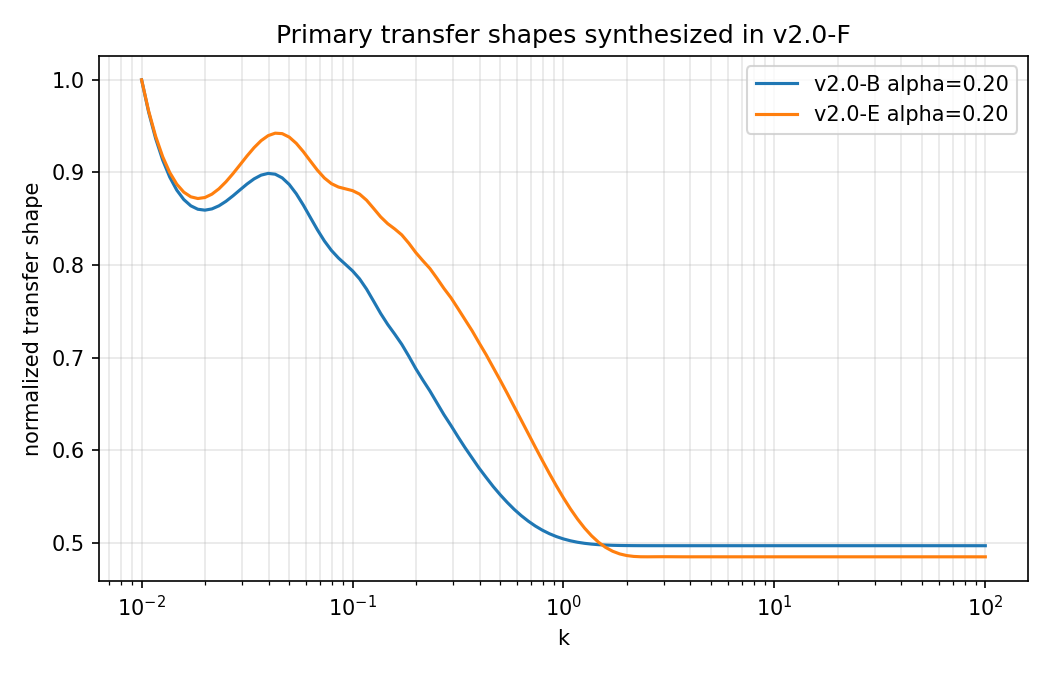
\includegraphics[width=0.88\linewidth]{../figures/SCT_v2_0_G_primary_transfer_comparison.png}
\caption{Primary transfer shapes synthesized in v2.0-F and included here for public readability. Both primary cases approach a bounded high-$k$ plateau rather than an indefinitely decaying Gaussian exponential.}
\end{figure}

\section{Interpretation}
The two tested closed-background routes do not support the Gaussian/diffusive transfer ansatz as a derived output. The result is stronger than the v1.7-v1.9 obstruction survey because it comes from preregistered numerical execution, not only from requirements inspection.

The correct conclusion is limited:
\begin{quote}
The Gaussian/diffusive ansatz $\exp[-(k/k_c)^2]$ is not supported by the two preregistered closed-background toy families tested in v2.0-B and v2.0-E.
\end{quote}

The result should not be overstated. It does not falsify all cyclic or bounce backgrounds. It does not derive a physical kernel. It does not establish a general no-go theorem. It does not address open-system kernels, stochastic noise, entropy production, or a physical restart mechanism.

\section{Claim boundary}
Allowed public claims:
\begin{itemize}[leftmargin=1.4em]
\item v2.0 refocused SCT onto a minimal computational transfer test.
\item Two toy background families were preregistered before execution.
\item Both produced non-Gaussian, bounded/high-$k$ plateau transfer shapes.
\item The current minimal closed-background $T_R$ route is closed as a limited negative computational result.
\end{itemize}

Forbidden claims:
\begin{itemize}[leftmargin=1.4em]
\item no general no-go theorem for cyclic or bounce cosmology;
\item no observational claim;
\item no physical cosmology claim;
\item no derivation of $P_\xi$, $\Gamma_S$, FDT/KMS, bath physics, entropy map, or restart dynamics;
\item no claim that SCT as an informational framework is falsified.
\end{itemize}

\section{Release note}
For public release, v2.0 should be presented as an addendum or synthesis package, not as a replacement for the full v1.6/v1.9 internal archive. A flat release package should include this addendum, the result tables, the execution scripts from v2.0-B and v2.0-E, and a hash ledger. Recursive internal recovery packages should remain internal.

\section*{Lineage anchors}
This addendum summarizes the local artifacts v1.9-R and v2.0-A through v2.0-F. Hashes are recorded in the accompanying lineage hash ledger. This document is not peer reviewed.

\end{document}
